\documentclass{article}
\usepackage[UTF8]{ctex}
\usepackage{amsmath,mathtools,geometry,pgfplots,float,mathrsfs,caption,enumerate}
\pgfplotsset{compat=1.15}
\usetikzlibrary{arrows}
\geometry{scale=0.7}

\title{每日一题(16.2)}
\author{\kaishu 程昊一}
\date{2022年5月11日}

\begin{document}
\maketitle
\begin{enumerate}
	\renewcommand{\labelenumi}{\textbf{\theenumi. }}
	\item 如图, $\triangle ABC$内有一点$P$, $AP$, $BP$, $CP$分别交$BC$, $CA$, $AB$于$D$, $E$, $F$. 证明:
	\[\frac{AE}{EC}\cdot\frac{CD}{DB}\cdot\frac{BF}{FA}=1.\]
	
	\item 如图, $\triangle ABC$内有一点$P$, 连接$AP$, $BP$, $CP$. 证明:
	\[\frac{\sin\alpha_1}{\sin\alpha_2}\cdot\frac{\sin\beta_1}{\sin\beta_2}\cdot\frac{\sin\gamma_1}{\sin\gamma_2}=1.\]
	(提示: 正弦定理)
	\begin{figure}[htbp]
		\centering
		\begin{minipage}[c]{0.48\textwidth}
			\centering
			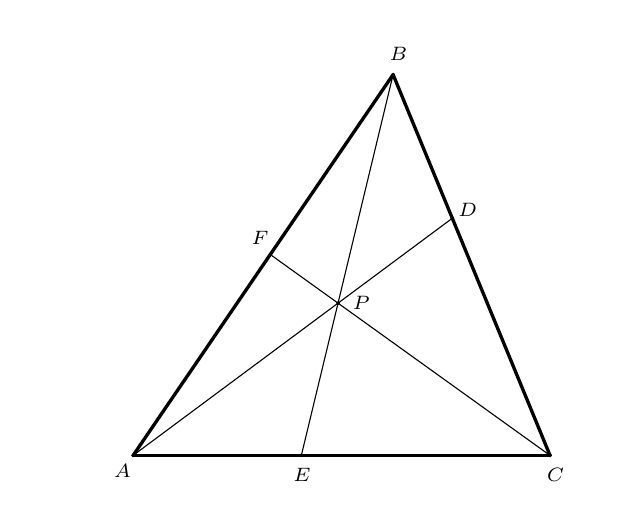
\begin{tikzpicture}[line cap=round,line join=round,>=triangle 45,x=1.0cm,y=1.0cm]
				\clip(-1.3391932575108423,-0.5) rectangle (6.029174564438354,5.432318131889642);
				\draw [line width=1.2pt] (0.,0.)-- (3.3017764239259417,4.836441534710075);
				\draw [line width=1.2pt] (3.3017764239259417,4.836441534710075)-- (5.2946118379360865,0.);
				\draw [line width=1.2pt] (5.2946118379360865,0.)-- (0.,0.);
				\draw [line width=0.4pt] (3.3017764239259417,4.836441534710075)-- (2.1365197847341344,0.);
				\draw [line width=0.4pt] (0.,0.)-- (4.053560426603639,3.0119258972824805);
				\draw [line width=0.4pt] (5.2946118379360865,0.)-- (1.7419867885406295,2.5516619465700954);
				\begin{scriptsize}
					\draw [fill=black] (0.,0.) circle (0.5pt);
					\draw[color=black] (-0.13458554942108222,-0.19258735249559444) node {$A$};
					\draw [fill=black] (3.3017764239259417,4.836441534710075) circle (0.5pt);
					\draw[color=black] (3.3703464825914966,5.095436315220471) node {$B$};
					\draw [fill=black] (5.2946118379360865,0.) circle (0.5pt);
					\draw[color=black] (5.364414609542343,-0.24703289862394517) node {$C$};
					\draw [fill=black] (2.6024039956129474,1.9336699505292638) circle (0.5pt);
					\draw[color=black] (2.9007536472344713,1.9375946397761283) node {$P$};
					\draw [fill=black] (2.1365197847341344,0.) circle (0.5pt);
					\draw[color=black] (2.145321694703605,-0.24703289862394517) node {$E$};
					\draw [fill=black] (4.053560426603639,3.0119258972824805) circle (0.5pt);
					\draw[color=black] (4.248280913911152,3.1149795748017133) node {$D$};
					\draw [fill=black] (1.7419867885406295,2.5516619465700954) circle (0.5pt);
					\draw[color=black] (1.6144776199521853,2.7610835249674333) node {$F$};
				\end{scriptsize}
			\end{tikzpicture}
			\caption*{\kaishu 第1题图}
		\end{minipage}
		\begin{minipage}[c]{0.48\textwidth}
			\centering
			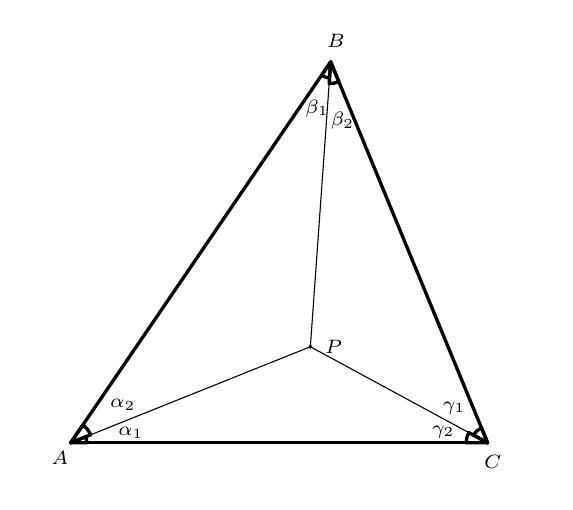
\begin{tikzpicture}[line cap=round,line join=round,>=triangle 45,x=1.0cm,y=1.0cm]
				\clip(-0.546457552431268,-0.5) rectangle (6.021910269517926,5.271914892710262);
				\draw [shift={(0.,0.)},line width=1.2pt] (0,0) -- (0.:0.2041707979813152) arc (0.:21.835881234897684:0.2041707979813152) -- cycle;
				\draw [shift={(0.,0.)},line width=1.2pt] (0,0) -- (21.83588123489768:0.27222773064175365) arc (21.83588123489768:55.67914927950503:0.27222773064175365) -- cycle;
				\draw [shift={(3.3017764239259417,4.836441534710075)},line width=1.2pt] (0,0) -- (-124.32085072049497:0.2041707979813152) arc (-124.32085072049497:-94.08178631031359:0.2041707979813152) -- cycle;
				\draw [shift={(3.3017764239259417,4.836441534710075)},line width=1.2pt] (0,0) -- (-94.08178631031357:0.27222773064175365) arc (-94.08178631031357:-67.60609570041895:0.27222773064175365) -- cycle;
				\draw [shift={(5.2946118379360865,0.)},line width=1.2pt] (0,0) -- (112.39390429958107:0.2041707979813152) arc (112.39390429958107:151.55046768077162:0.2041707979813152) -- cycle;
				\draw [shift={(5.2946118379360865,0.)},line width=1.2pt] (0,0) -- (151.55046768077162:0.27222773064175365) arc (151.55046768077162:180.:0.27222773064175365) -- cycle;
				\draw [line width=1.2pt] (0.,0.)-- (3.3017764239259417,4.836441534710075);
				\draw [line width=1.2pt] (3.3017764239259417,4.836441534710075)-- (5.2946118379360865,0.);
				\draw [line width=1.2pt] (5.2946118379360865,0.)-- (0.,0.);
				\draw [line width=0.4pt] (3.0436732058213924,1.219594000208503)-- (3.3017764239259417,4.836441534710075);
				\draw [line width=0.4pt] (3.0436732058213924,1.219594000208503)-- (0.,0.);
				\draw [line width=0.4pt] (3.0436732058213924,1.219594000208503)-- (5.2946118379360865,0.);
				\begin{scriptsize}
					\draw [fill=black] (0.,0.) circle (0.5pt);
					\draw[color=black] (-0.13767904636019296,-0.19382475127123847) node {$A$};
					\draw [fill=black] (3.3017764239259417,4.836441534710075) circle (0.5pt);
					\draw[color=black] (3.3672529856523843,5.1010046097108726) node {$B$};
					\draw [fill=black] (5.2946118379360865,0.) circle (0.5pt);
					\draw[color=black] (5.36132111260323,-0.2482702973995892) node {$C$};
					\draw [fill=black] (3.0436732058213924,1.219594000208503) circle (0.5pt);
					\draw[color=black] (3.3400302125882093,1.2217594480658813) node {$P$};
					\draw[color=black] (0.7640753113906159,0.12708553172815106) node {$\alpha_1$};
					\draw[color=black] (0.6619899123999583,0.4833417287001241) node {$\alpha_2$};
					\draw[color=black] (3.130096420836179,4.246890104822371) node {$\beta_1$};
					\draw[color=black] (3.4531583110741955,4.085638865427976) node {$\beta_2$};
					\draw[color=black] (4.86999374980571,0.4445929680945187) node {$\gamma_1$};
					\draw[color=black] (4.7317944854941745,0.13833677112254567) node {$\gamma_2$};
				\end{scriptsize}
			\end{tikzpicture}
			\caption*{\kaishu 第2题图}
		\end{minipage}
		
	\end{figure}
	
\end{enumerate}
\end{document}